\documentclass[11pt, a4paper]{article}

\usepackage{listings}
\usepackage{color}
\usepackage[normalem]{ulem}
\usepackage{graphicx}
\usepackage{hyperref}


\definecolor{dkgreen}{rgb}{0,0.6,0}
\definecolor{gray}{rgb}{0.5,0.5,0.5}
\definecolor{mauve}{rgb}{0.58,0,0.82}

\lstset{frame=tb,
  language=SQL,
  aboveskip=3mm,
  belowskip=3mm,
  showstringspaces=false,
  columns=flexible,
  basicstyle={\small\ttfamily},
  numbers=none,
  numberstyle=\tiny\color{gray},
  keywordstyle=\color{blue},
  commentstyle=\color{dkgreen},
  stringstyle=\color{mauve},
  breaklines=true,
  breakatwhitespace=true
  tabsize=3
}

\begin{document}
\title{}
\author{Groep A\\ Rapport 1}
\date{19 maart 2014}
\maketitle

\section{Status}
Het project is afgewerkt. Alle verplichte functionaliteit is afgewerkt en we hebben heel wat extra functionaliteit voorzien. De database is goed gevuld met ongeveer 86.000 entries. De afgewerkte versie van de website staat online op \url{www.coachcenter.be / www.coachcenter.net} en blijft automatisch up to date met de recentste data.
\section{Taakverdeling}
In deze sectie noemen we enkel de grote onderdelen waar we veel aan werkten. Dit is verre van een complete lijst. Voor een vollediger beeld is er het overzicht van de commits op onze git repository \\ \url{https://github.com/rubenvanassche/Programming-Project-Databases}
\subsection{Stijn}
Was verantwoordelijk voor het binnenhalen alle voetbalgerelateerde data (door middel van crawler), dit ging van matchen (zowel de nog te spelen als de gespeelde), competities, info over de matchen zoals spelers, kaarten, doelpunten, en spelerwissels, teams en zijn spelers, FIFA rank,... Uiteraard zou de design voldoende robuust moeten zijn en bovendien efficiënt genoeg zodat het geen eeuwigheid zou duren voordat de net gespeelde matchen weer up-to-date is.
\subsection{Kristof}
Heeft enkele pagina's gemaakt en ook de back-end verzorgd die nodig was voor die pagina's. Heeft de basis gelegd voor user profiles en  heeft private usergroups gemaakt. Bouwde een notificatiesysteem en zorgde ook voor de email reminders. 
\subsection{Tom}
Maakte de algoritmen die aan de hand van de data in de database een beredeneerde calculatie moest maken over de uitslag van de wedstrijden.
Zorgde voor het sorteersysteem en filtersysteem van de tabellen.
\subsection{Jakob}
Maakte een gebruikerssysteem (registreren en inloggen). Maakte een interactieve wereldkaart met FIFA scores. Bouwde het betsysteem uit. Maakte een visualisatie van statistieken uit de database.
\subsection{Ruben}


\section{Design}
TODO: LAMP, Laravel, Bootstrap
\subsection{Voorspellingsalgoritme}
Het voorspellingssysteem hebben wij opgesplitst in 2 essenti\"ele delen, namelijk het voorspellen van een winnaar van een wedstrijd, en het bepalen van de te verwachten score. Factoren die wij belangrijk vonden om rekening mee te houden in het voorspellen van dit alles zijn vooral onderlinge resultaten van eerder gespeelde wedstrijden, en gemiddeldes van andere wedstrijden tegen andere ploegen. Ook wordt altijd rekening gehouden met de locatie waar gespeeld wordt (uit of thuis).
\\
\\
Het voorspellen van de winnaar is natuurlijk de makkelijkste van de twee. We beginnen simpelweg door te kijken naar eerder gespeelde wedstrijden tussen deze ploegen. We werken met een puntensysteem waarbij een ploeg punten krijgt wanneer het een wedstrijd wint. Het aantal punten dat het krijgt, hangt af van de impact die we willen dat het heeft op het gehele resultaat. Hierbinnen maken we ook nog eens het onderscheid of de set-up uit/thuis dezelfde is of omgekeerd. Het eerste geval is natuurlijk het belangrijkste aangezien dit een identieke case is. Daarom zal een ploeg ook de meeste punten worden toegekend voor het winnen van zulke wedstrijden.
Daarna gaan we kijken naar algemene resultaten, maar weer rekening houdende met het al dan niet uit/thuis spelen. We kijken naar alle wedstrijden die de thuisploeg thuis speelde, en de uitploeg uit speelde. Voor elke gewonnen match krijgen ze ieder weer een bepaald aantal punten (afhankelijk van de impact die deze factor moet hebben). Vervolgens kijken we naar de wedstrijden waar de thuisploeg uit speelde, en de uitploeg thuis. Wederom krijgen ze voor iedere gewonnen match een bepaald aantal punten maar weer minder dan in het vorige geval. Tot slot gaan we de punten vergelijken en op basis daarvan kunnen we de kans bepalen dat een bepaalde ploeg wint.
\\
\\
Het bepalen van een score is iets complexer. Dit volgt een gelijkaardig systeem als hierboven, maar met een belangrijk verschil. Hier werken we niet met het optellen van punten. We gaan altijd werken met gemiddeldes. Zo zullen we wederom eerst kijken naar identieke wedstrijden en van elke ploeg het gemiddelde aantal goals bewaren. Dan gaan we kijken naar wedstrijden met dezelfde ploegen maar op een andere locatie en wederom berekenen we het gemiddeld aantal goals gescoord door de teams.
Dan gaan we weer kijken naar de algemene resultaten waarbij we wel wederom een onderscheid maken tussen uit- en thuis spelen. We berekenen dus het gemiddelde aantal goals dat de thuisploeg thuis scoort, en het gemiddelde aantal goals dat de thuisploeg uit scoort. Voor de uitploeg natuurlijk net hetzelfde. Nu zitten we met 4 gemiddeldes die we individueel vermenigvuldigen met een factor (mate van impact) en daarna optellen en delen door 4. Door dit af te ronden hebben we nu een aantal goals bepaald voor iedere ploeg. Op het einde van dit algoritme zit ook nog een systeem dat ons zal verzekeren dat de kansen van winst overeen komt met de berekende score. Ook hebben we een bepaalde marge berekend van 10\% voor gelijkspel. Op deze manier zal het resultaat van de kansberekening nooit in tegenspraak zijn met de berekende score.
\\
\\
Eerst hadden we ook de bedoeling om nog meer dingen te laten berekenen aan de hand van de data die we hebben. Maar al snel bleek dat deze dingen vaak te willekeurig zijn en daarom konden er ook niet echt beredeneerde gokken over worden gemaakt. Er zijn inderdaad wel spelers die vaker kaarten krijgen dan andere, maar uiteindelijk blijkt dit toch veelal willekeurig te zijn. Al snel bleek dat een algoritme hiervoor vaker ernaast zou zitten dan erop. Om onze gebruiker dan ook niet het valse gevoel te geven van hierop te kunnen gokken aan de hand van dit algoritme, hebben we besloten het niet in het uiteindelijke project te steken.

\subsection{Voorspellingen van gebruikers}
Via een formulier kunnen gebruikers voorspellingen uitbrengen. Dit formulier kan zowel bereikt worden via het gebruikersmenu bovenaan elke pagina, of via een knop op de pagina's van matchen. In het tweede geval worden teams en datum uiteraard al voor de gebruiker ingevuld. De gebruiker kan verder voorspellingen uitbrengen over de eindscore, wie het eerste doelpunt scoort, hoeveel gele kaarten elk team krijgt en hoeveel rode kaarten elk team krijgt. Dit kan later makkelijk uitgebreid worden. Voorspellen van eindscore is verplicht, de rest kan de gebruiker naar eigen wil blanco laten. Indien geen goals gescoord worden, dient er uiteraard niet opgegeven te worden wie het eerste doelpunt scoort.	Om te kunnen bepalen wie de beste voorspellingen uitbracht, krijgt elke speler een puntentotaal afhankelijk van zijn voorspellingen. Dit zal afhankelijk zijn van de correctheid van voorspellingen en het aantal uitgebrachte voorspellingen. Merk op dat hoe meer dingen een gebruiker voorspelt, hoe meer punten er voor die match te verdienen zijn, maar hoe minder punten er per afzonderlijke voorspelling te verdienen zijn. Op deze manier is het invullen van extra voorspellingen een risk-rewardsituatie. We willen vermijden dat iedereen zich verplicht voelt alles in te vullen omdat ze anders geen kans maken, maar ook dat niemand extra voorspellingen invult omdat het nooit de moeite loont. Om de precieze afwegingen te bepalen zullen we nog wat moeten experimenteren. Het is momenteel mogelijk om voorspellingen uit te brengen, gemaakte voorspellingen te bekijken en de correctheid van voorspellingen van ondertussen gespeelde wedstrijden na te gaan, maar puntentellingen en vergelijkingen met andere gebruikers gebeuren nog niet. Ook worden voorspellingen van het systeem nog niet getoond.
\\
Momenteel is het mogelijk om voorspellingen uit te voeren op reeds gespeelde matchen. In de uiteindelijke versie van de site zal dit natuurlijk niet meer nodig zijn, maar nu kan dit nog, met oog op demo'en van functionaliteit zonder een halve dag te moeten wachten en bugfixen. Momenteel worden nog geen punten geteld op basis van voorspellingen, en we zullen de gemaakte voorspellingen nog resetten eens dat wel gebeurt. Zo geeft deze optie geen oneerlijk voordeel aan early adopters van onze site.
\\
Gemaakte voorspellingen worden opgeslagen in een specifieke tabel, `bet`, in de database. Concreet krijgt elke voorspelling een unieke id, en worden id van match en gebruiker en alle gemaakte voorspellingen bijgehouden.

\section{Database}
TODO: UPDATE
Onze database bestaat 20 tabellen met voetbalgerelateerde data en 2 usergerelateerde tabellen.
\begin{enumerate}
\item 'continent': Tabel voor werelddelen. Bevat een id en een naam.
\item `country`: Tabel voor landen. Bevat een id, een naam, de id van het werelddeel waarin het land ligt, en een afkorting voor de naam van het land. Die afkorting zal gebruikt worden op de website.
\item `player`: Tabel voor voetbalspelers. Bevat een id, een naam en een boolean die aangeeft of de speler geblesseerd is.
\item `coach`: Tabel voor voetbalcoaches. Bevat een id en een naam.
\item `team`: Tabel voor voetbalteams. Bevat een id, een naam, een id van het land van het team, een id van de huidige coach van het team en de FIFA score.
\item `competition`: Tabel voor voetbalcompetities. Bevat een id en een naam.
\item `match`: Tabel voor voetbalmatches. Bevat id's van thuis- en uitteam, id van de competitie en een datum.
\item `playerPerTeam`: Tabel die spelers en teams met elkaar linkt. Bevat id's van een speler en een team.
\item `playerPerMatch`: Tabel die spelers en matches met elkaar linkt. Bevat id's van een speler en een match en de tijden waarop de speler op het veld kwam en van het veld ging.
\item `teamPerCompetition`: Tabel die teams en competities met elkaar linkt. bevat id's van een team en een competitie.
\item `goal`: Tabel voor doelpunten. Bevat id van match waarin doelpunt gescoord is, tijdstip waarop, id van de speler die het doelpunt scoorde, id van het team waarnaar het punt ging en een boolean die aangeeft of het doelpunt tijdens de penaltyfase gescoord werd.
\item `cards`: Tabel voor gele en rode kaarten. Bevat een id, een id van de speler die de kaart kreeg, een id van de match waarin de kaart gegeven werd, de kleur van de kaart en de tijd waarop de kaart gegeven werd.
\item `user`: Meer uitleg bij sectie over gebruikers.
\item `bet`: Meer uitleg bij sectie over voorspellingen
\item `notifications`: Meer uitleg bij sectie over notifications
\item `userGroup`: Meer uitleg bij sectie over user groups
\item `userGroupInvites`: Meer uitleg bij sectie over user groups
\item `userGroupMessages`: Meer uitleg bij sectie over user groups
\item `userGroupMessagesContent`: Meer uitleg bij sectie over user groups
\item `userPerUserGroup`: Meer uitleg bij sectie over user groups

\end{enumerate}

\subsection{ER-diagramma}
Zie laatste pagina
\subsection{Relational model}
continent(\uline{id}, name) \\
country(\uline{id}, name, continent\_id, abbreviation) \\
player(\uline{id}, name) \\
coach(\uline{id}, name) \\
team(\uline{id}, name, country\_id, coach\_id, fifapoints, twitterAccount) \\
competition(\uline{id}, name) \\
match(\uline{id}, hometeam\_id, awayteam\_id, competition\_id, date) \\
playerPerTeam(\uline{player\_id}, \uline{team\_id}, position) \\
playerPerMatch(\uline{player\_id}, \uline{match\_id}, intime, outtime) \\
teamPerCompetition(\uline{team\_id}, \uline{competition\_id}) \\
goal(match\_id, time, player\_id, team\_id) \\
cards(\uline{id}, player\_id, color, time) \\
user(\uline{id}, facebookid, username, firstname, lastname, email, password, country\_id, session\_id, registrationcode, betscore, about, receive\_email, age, picture) \\
bet(\uline{id}, user\_id, match\_id, hometeam\_score, awayteam\_score, first\_goal, hometeam\_yellows, hometeam\_reds, awayteam\_yellows, awayteam\_reds, evaluated, betdate) \\
notifications(\uline{id}, actor\_id, subject\_id, object\_id, type\_id, status, created\_date, updated\_date) \\
userGroup(\uline{id}, name, private, created) \\
userGroupInvites(\uline{id}, user\_id, usergroup\_id, invitedby\_id, created) \\
userGroupMessages(\uline{id}, usergroup\_id, user\_id, title, created) \\
userGroupMessagesContent(\uline{id}, user\_id, message\_id, content, created) \\
userPerUserGroup(\uline{user\_id}, \uline{usergroup\_id}, created)\\

\subsection{Constraints}
\begin{lstlisting}
-- Constraints for table `cards`
--
ALTER TABLE `cards`
  ADD CONSTRAINT `match` FOREIGN KEY (`match_id`) REFERENCES `match` (`id`) ON DELETE NO ACTION ON UPDATE CASCADE,
  ADD CONSTRAINT `player` FOREIGN KEY (`player_id`) REFERENCES `player` (`id`) ON DELETE CASCADE ON UPDATE CASCADE;

--
-- Constraints for table `country`
--
ALTER TABLE `country`
  ADD CONSTRAINT `continent` FOREIGN KEY (`continent_id`) REFERENCES `continent` (`id`);

--
-- Constraints for table `goal`
--
ALTER TABLE `goal`
  ADD CONSTRAINT `goal_match` FOREIGN KEY (`match_id`) REFERENCES `match` (`id`) ON DELETE NO ACTION ON UPDATE CASCADE,
  ADD CONSTRAINT `goal_player` FOREIGN KEY (`player_id`) REFERENCES `player` (`id`) ON DELETE NO ACTION ON UPDATE CASCADE,
  ADD CONSTRAINT `goal_team` FOREIGN KEY (`team_id`) REFERENCES `team` (`id`) ON DELETE NO ACTION ON UPDATE CASCADE;

--
-- Constraints for table `match`
--
ALTER TABLE `match`
  ADD CONSTRAINT `awayteam` FOREIGN KEY (`awayteam_id`) REFERENCES `team` (`id`) ON DELETE CASCADE ON UPDATE CASCADE,
  ADD CONSTRAINT `hometeam` FOREIGN KEY (`hometeam_id`) REFERENCES `team` (`id`) ON DELETE CASCADE ON UPDATE CASCADE,
  ADD CONSTRAINT `match_competition` FOREIGN KEY (`competition_id`) REFERENCES `competition` (`id`);

--
-- Constraints for table `playerPerMatch`
--
ALTER TABLE `playerPerMatch`
  ADD CONSTRAINT `player_per_match` FOREIGN KEY (`match_id`) REFERENCES `match` (`id`) ON DELETE CASCADE ON UPDATE CASCADE;

--
-- Constraints for table `playerPerTeam`
--
ALTER TABLE `playerPerTeam`
  ADD CONSTRAINT `player_per_team` FOREIGN KEY (`team_id`) REFERENCES `team` (`id`) ON DELETE CASCADE ON UPDATE CASCADE;

--
-- Constraints for table `team`
--
ALTER TABLE `team`
  ADD CONSTRAINT `team_coach` FOREIGN KEY (`coach_id`) REFERENCES `coach` (`id`) ON DELETE NO ACTION ON UPDATE CASCADE,
  ADD CONSTRAINT `team_country` FOREIGN KEY (`country_id`) REFERENCES `country` (`id`);

--
-- Constraints for table `teamPerCompetition`
--
ALTER TABLE `teamPerCompetition`
  ADD CONSTRAINT `tpc_competition` FOREIGN KEY (`competition_id`) REFERENCES `competition` (`id`);

  --
-- Constraints for table `bet`
--
ALTER TABLE `bet`
  ADD CONSTRAINT `matchID` FOREIGN KEY (`match_id`) REFERENCES `match` (`id`) ON DELETE CASCADE ON UPDATE CASCADE,
  ADD CONSTRAINT `userID` FOREIGN KEY (`user_id`) REFERENCES `user` (`id`) ON DELETE NO ACTION ON UPDATE CASCADE;

\end{lstlisting}

\section{User interface}

Hoewel Laravel beschikt over een volledig uitgewerkt loginsysteem, besloten we ons eigen systeem te schrijven. Een dergelijk systeem gebruikt een database voor het opslaan van users, dus is het niet meer dan logisch dat we dit in een vak met betrekking tot databases zelf gaan programmeren. In de database bestaat een tabel 'user', met als fields 'id', 'username', 'firstname', 'lastname', 'email', 'password', 'country\_id', 'session\_id', 'registrationcode', 'betscore', 'about', 'receive\_email', 'age' en 'picture' . De id is een auto incrementing integer die dient als key voor elke entry van de tabel. We voorzien een username, zodat gebruikers niet noodzakelijk hun echte naam moeten prijsgeven. Daarnaast is het een makkelijke manier om gebruikers op de website een unieke benaming te geven. Voornaam en familienaam zijn apart opgeslagen, zodat we in bijvoorbeeld emails gebruikers niet altijd met hun volledige naam niet hoeven aan te spreken. Het paswoord is uiteraard gehasht opgeslagen. Het hashen gebeurt via Laravel, aan de hand van bcrypt. Bcrypt is gebaseerd op het Blowfishalgoritme en heeft een salt ingebouwd, wat accounts beschermt tegen aanvallen gebruik makende van rainbow tables. Laravel biedt een functie voor het vergelijken van een ongehasht en gehasht paswoord. Verder vragen we gebruikers ook in welk land ze wonen en wat hun leeftijd is. De session\_id wordt gebruikt om bij te houden of een gebruiker ingelogd is. We plaatsen een tijdelijke cookie met hetzelfde id bij de gebruiker, en kunnen dit zo nagaan. De registratiecode wordt gebruikt bij het nagaan van de validiteit van het emailadres van een gebruiker. De registratiecode wordt gemaild naar de gebruiker, en het account wordt pas geactiveerd wanneer deze code ingegeven wordt. De betscore houdt bij hoe goed een gebruiker presteert bij het gokken. De gebruiker kan een korte beschrijving van zichzelf geven, die in 'about' wordt opgeslagen. 'Receive\_email' is een boolean die bijhoudt of de gebruikers herinneringse-mails voor wedstrijden waar hij nog niet op gokte wil krijgen. Ten slotte bevat 'picture' de profielafbeelding van de gebruiker.
\\
\\
Voor de validatie van input bij registreren (zijn verplichte velden ingevuld, staat bij emailadres wel een emailadres, is tweemaal hetzelfde paswoord ingetypt, ...) is de validatie van Laravel gebruikt. Dergelijke validatiecode ziet er heel wat beter uit voor de programmeur dan via een hoop simpele if-statements en reguliere expressies. We gebruiken de Laravel Query Builder voor makkelijker schrijven van SQL queries niet, dit gebeurt zoals opgegeven met ruwe SQL queries.
\\
\\
Op elke webpagina verschijnt voor een niet-ingelogde gebruiker een loginknop. Het loginmenu wordt dan over de huidige pagina (in een 'modal', een feature van Bootstrap) weergegeven. Indien de gebruiker met foute gegegvens probeert in te loggen, wordt dit afgehandeld in diezelfde modal. Eens inloggen succesvol is, verschijnt er in de modal nog een bericht om het inloggen te bevestigen. Eens dat weggeklikt wordt, bevindt de gebruiker zich terug op dezelfde pagina als voorheen. In de modal "forgot password"-functionaliteit voorzien. De gebruiker geeft zijn emailadres in, en er wordt een email gestuurd waarmee het paswoord gereset kan worden. Indien men probeert in te loggen met een account waarvan het emailadres nog niet gevalideerd is, verschijnt een knop om de activatiemail opnieuw te versturen. \\ Bij een ingelogde gebruiker wordt bij elke bezochte pagina de login cookie gerefresht, zodat een gebruiker bij langdurige sessies op de site niet om de zoveel tijd opnieuw hoeft in te loggen. \\ \\

TODO: Facebooklogin \\ \\

Eens ingelogd, worden de registratie- en inlogknoppen vervangen door "My Profile", "Bets", "Preferences" en "Logout". \\
"My Profile" is een pagina waarop wat persoonlijke informatie als land en bet score te zien zijn. Deze pagina is voor iedereen, zelfs niet-ingelogde gebruikers zichtbaar. Enkel op je eigen profiel verschijnen nog de tabs "Notifications", "My Groups" en "Invitations". Op deze functionaliteit wordt verder ingegaan in andere secties. \\
Onder "Preferences" is het mogelijk je persoonlijke gegevens aan te passen.	Ook is er een opt-out voor herinneringsemails omtrent bets. Uploaden van profielafbeeldingen gebeurt ook daar.
Als de gebruiker op "logout" klikt, wordt hij uitgelogd en naar de homepage gestuurd. \\ \\

Uitgelogde gebruikers zullen niet gelinkt worden naar pagina's voor enkel gebruikers. Indien iemand toch probeert een dergelijke pagina te bezoeken door de URL in te typen, zal hij gevraagd worden eerst in te loggen of te registreren en de eigenlijke pagina niet te zien krijgen. \\ \\

\subsection{Betsysteem}
Gebruikers kunnen pronostieken invullen voor matchen in de toekomst. Voor een ingelogde gebruiker verschijnt op matchpagina's een knop genaamd "bet", zolang de gebruiker nog niet eerder een gok heeft uitgebracht op die match. Wanneer de gebruiker erop klikt, verschijnt het betformulier in een modal. De gebruiker is verplicht om een eindscore in te vullen. Eerste goal en aantallen kaarten zijn optioneel. De gok wordt geregistreerd van zodra er op "bet" geklikt wordt. Elke gebruiker heeft per match slechts \'e\'en kans per match, denk dus goed na over je bet. Een overzicht van gemaakte bets kan gevonden worden via "bets" in de bovenste balk op de website. Daar worden bets opgedeeld in bets op toekomstige matchen en bets op verleden matchen. Er kan telkens doorgeklikt worden naar de matchen en teams. \\ \\
Eens een match gespeeld is, worden de bets erop binnen de drie uur ge\"evalueerd. Aan elke gebruiker wordt een aantal punten toegekend. Dat puntentotaal kan ook negatief zijn. Er kan met elke gemaakte gok een aantal punten gewonnen of verloren worden. Er kunnen altijd meer punten gewonnen worden dan verloren. Eerst hadden we het idee om correcte riskante gokken meer punten waard te maken. We waren van plan om "riskante gokken" te defini\"eren als keuzes waar weinig gebruikers voor gingen. Realistisch gezien zullen er waarschijnlijk niet erg veel gebruikers actief zijn tijdens het WK 2014 en zou een dergelijk systeem niet erg veel nut hebben. Daarom hebben we per optie een vast aantal punten toegekend (maar niet voor elke optie evenveel). \\ \\

\subsection{Filter- & sorteersysteem}
Ook kunnen gebruikers zowat elke tabel die te vinden is op de website sorteren zoals zij dit zelf willen. Dit hebben we verwezenlijkt met een slim stukje javascript dat een uitbreiding is op tablesorter. Hierdoor moet de webpagina niet opnieuw geladen worden. Ook is er een ingebouwd filter systeem waardoor de gebruiker op een overzichtelijke en snelle manier ervoor kan zorgen dat alleen de data die hij relevant is voor hem zichtbaar is.
Al deze functionaliteit zou moeten bijdragen aan de gebruiksvriendelijkheid van de website. Ook hebben we dit alles zo intiutief mogelijk gehouden zodat de gebruiker zonder enig probleem kan navigeren over de website en zich meer kan concentreren op de inhoud dan hoe hij daar moet geraken.



\subsection{Notificaties}
Ook is er in ons systeem een uitgebreid notificatiesysteem aanwezig. Wanneer een gebruiker ingelogd is, zal er bovenaan naast het user menu een nieuw item tevoorschijn komen (icoon: ster). Op het moment dat er een notificatie is voor de gebruiker wordt die hier getoond. Zonder op het item te klikken kan je al zien hoeveel ongelezen notificaties je hebt door het cijfer in superscript dat naast het sterretje staat. Als de gebruiker hierop klikt komt er een dropdown menu tevoorschijn met de meest recente notificaties. Deze notificaties linken naar de relevante pagina. \\
Om dit mogelijk te maken is er een notificatiesysteem geschreven dat gemakkelijk uitbreidbaar is. Elke notificatie heeft een specifiek formaat: er is altijd een actor, een subject, een object en een type. Aan de hand van deze informatie kan er dan een gepaste boodschap worden getoond.
\begin{enumerate}
\item Actor: de uitvoerende partij
\item Subject: de persoon voor wie de notificatie bestemd is
\item Object: de specifieke informatie over de notificatie
\item Type: om duidelijk te maken welk voor type notificatie we hebben (Bijvoorbeeld een usergroup invite)
\end{enumerate}
\subsubsection{Implementatie}
Elke notificatie komt dus overeen met een rij van de notifications table. Wanneer een notificatie wordt opgeslagen (Notifications::saveNotification) komt er niet veel bij zien: gewoon letterlijk de kolommen invullen.
Bij het opvragen van een notificatie (Notifications::getNotification) komt er wat meer bij kijken: in het resultaat wordt de informatie van het object erbij gezet.
Wanneer er op de notificatie wordt geklikt wordt de redirect methode van de NotificationController opgeroepen die naargelang het type notificatie de gebruiker naar de juiste pagina redirect.

\subsection{Soorten notificaties}
\subsubsection{Usergroup invites}
Een gebruiker nodigt een andere gebruiker uit om een usergroup te joinen.
\begin{enumerate}
\item Actor: de gebruiker die de persoon uitnodigt
\item Subject: de uitgenodigde gebruiker
\item Object: de userGroupInvite
\item Type: 1, Notifications::INVITE\_USER\_GROUP
\end{enumerate}
De notificatie zal linken naar de gebruiker zijn profiel waar die de invitatie zal kunnen accepteren of weigeren.

\subsubsection{Remind user bets}
Het systeem herinnert de gebruikers om te betten op matchen waar ze dat nog niet op hebben gedaan.
Omdat het systeem dit verstuurt zullen we de actor en subject dezelfde personen nemen.
\begin{enumerate}
\item Actor: de gebruiker
\item Subject: de gebruiker
\item Object: NULL (Geen verdere info nodig)
\item Type: 2, Notifications::REMIND\_USER\_BETS
\end{enumerate}
De notificatie zal linken naar de upcoming matches page, waar de gebruiker gemakkelijk kan zien op welke matches hij/zij nog niet op heeft gebet.

\subsubsection{Nieuwe discussie in usergroup}
Wanneer een gebruiker een nieuwe discussie start in een usergroup zullen alle members van die groep een notificatie hierover krijgen.
\begin{enumerate}
\item Actor: de gebruiker die de discussie heeft aangemaakt
\item Subject: een gebruiker die lid is van de groep
\item Object: de discussie
\item Type: 3, Notifications::NEW\_DISCUSSION
\end{enumerate}
De notificatie zal linken naar de discussie.

\subsubsection{Nieuwe reply in discussie}
Als een gebruiker een bericht post in de discussie zullen alle deelnemers van die discussie hierover genotified worden.
\begin{enumerate}
\item Actor: de gebruiker die een nieuwe reply heeft gemaakt
\item Subject: deelnemer aan de discussie
\item Object: discussie
\item Type: 4, Notifications::NEW\_MESSASGE
\end{enumerate}
De notificatie linkt naar de discussie.

\subsection{Email reminders}
Gebruikers worden tijdig herinnerd wanneer ze nog niet op bepaalde wedstrijden hebben gebet. Dit wordt mogelijk gemaakt door een combinatie van een Laravel command die via een cronjob om de zoveel tijd loopt.
Momenteel worden de gebruikers elke dag herinnerd om te wedden op de wedstrijden die de komende twee dagen worden gespeeld waar ze nog niet reeds hebben op gebet.
Ook wordt er een wekelijks overzicht gegeven op zondag met een overzicht van de wedstrijden die in de komende week worden gespeeld.

De functie die in het Laravel command wordt opgeroepen is de Notifications::sendReminders. Dit zal samen met een email ook een notificatie sturen naar de gebruiker.

Uiteraard moet de gebruiker de mogelijkheid krijgen om geen emails meer te ontvangen. Vandaar dat er ook een opt-out mogelijkheid is. Enerzijds kan je dit doen door op de link in de email te klikken,
anderzijds kan je dit regelen door de knop op de preferences page te gebruiken. Deze knop/link togglet als het ware tussen het ontvangen van email en het niet ontvangen van de mail. Als de gebruiker zich op een later moment
bedenkt kan deze dit dus gewoon via de preferences page (of een link in een email) regelen.

\subsection{Grafische weergave van statistieken}
Voor de grafische weergave van data gebruiken we Google Charts. Dat biedt heel wat verschillende grafieken. Momenteel zijn op elke teampagina twee grafieken beschikbaar. Er is een taartdiagram dat het percentage gewonnen, verloren en gelijkgespeelde matchen van een team toont. Ook is er een staafdiagram dat het gemiddelde aantal goals en/of kaarten per match per jaar toont. De gebruiker kan kiezen welke combinatie van 'gemiddeld aantal goals', 'gemiddeld aantal gele kaarten' en 'gemiddeld aantal rode kaarten' hij wil zien. De grafiek wordt meteen aangepast, zonder dat de pagina opnieuw geladen moet worden. Deze grafieken bevinden zich onder de tab 'Graphs' op elke teampagina. \\ \\
Op de homepagina staat een grote wereldkaart. De kleur van elk land geeft zijn FIFA score weer. Hoe donkerder het land, hoe hoger de score. Wanneer op een land geklikt wordt, wordt meteen naar de teampagina van het nationale team gelinkt. Voor enkele kleine landen is geen teampagina aanwezig, er gebeurt dan ook niets wanneer erop geklikt wordt. Als op het Verenigd Koninkrijk geklikt wordt, zoomt de kaart in, zodat op de vier aparte delen (Wales, Engeland, Noord-Ierland en Schotland) kan worden geklikt. Deze hebben namelijk elk een apart nationaal team. \\ \\
Ook de voorspellingen van het systeem worden gevisualiseerd. Concreet staat op elke matchpagina van toekomstige matchen een balk in twee kleuren. Het linkerdeel geeft de kans op winst voor de thuisploeg aan, het rechterdeel die voor de uitploeg. Deze balk is niet met Google Charts gemaakt, maar is een progress bar van Bootstrap.
\section{Webpagina's}
De gemaakte webpagina's zijn in het Laravel PHP Framework gemaakt. Dit is een framework dat MVC hoog in het vaandel draagt en dat proberen we dus ook te respecteren.
Elke pagina (View) heeft een controller tot zijn beschikking. Deze dient als tussenstuk tussen het model van de pagina waar de werkelijke queries gebeuren. Over het algemeen is dit wat er gebeurt:
\\
\\
Er wordt een pagina opgevraagd in de url. (Bv. /public/team/1). In de route-file wordt gedefinieerd welke controller er opgeroepen moet worden. Deze controller zal informatie opvragen van het
relevante model en zal deze info doorspelen naar de view van de pagina.
\\
\\
Aanvankelijk was het werken met het framework niet eenvoudig maar eens het wat duidelijker werd zagen we de waarde ervan in.
Het design hebben we grotendeels te danken aan Twitter Bootstrap. Een website ziet er zo relatief gemakkelijk goed uit.
\\
\\
\subsection{Home page}
Bestaat uit 3 tabellen, een news foto feed en een wereldkaart die de landen kleurt in functie van hun WK-ranking.
De 3 tabellen bevatten data over de laatst gespeelde matchen, de opkomende matchen en de fifa-ranking.
\\
De foto newsfeed is een RSS feed van FIFA die we met SimplePie hebben geparsed.
\\
Op de wereldkaart krijgt elk land een tint groen toegekend; hoe hoger hun WK-ranking, hoe donkerder het groen. Wanneer men op een land klikt zal de gebruiker gelinkt worden naar de desbetreffende team pagina van het nationale team van dat land. Merk op dat het Verenigd-Koninkrijk wegens beperkingen van de gebruikte Google GeoCharts-API niet ingekleurd is; zij hebben vier "nationale" teams (Engeland, Wales, Noord-Ierland, Schotland). Om dit op te lossen, wordt bij klikken op het VK ingezoomd, waarna de vier delen apart in de juiste kleur verschijnen.

\subsection{Search bar / search results}
Rechtsbovenaan alle pagina's staat een searchbar waarin je een zoekterm kunt invullen en die de beschikbare info (hetzij team/speler/match) presenteert. Als je op de links doorklikt word je doorgestuurd naar de desbetreffende pagina.

\subsection{Player Page}
Deze pagina bevat informatie over een bepaalde speler.
\\
In de PlayerController wordt volgende info opgevraagd van de Player en Team models:
Deze informatie wordt dan vervolgens gebruikt om weer te geven op de webpagina. Met andere woorden worden hun goals, kaarten etc. getoond. Wat wel opgemerkt moet worden is dat momenteel de playerText en de playerImageURL van wikipedia worden gehaald en niet
in onze database zitten.

\subsection{Team Page}
Deze pagina bevat informatie over een bepaald team, zoals de spelers, matchen e.d.
In de TeamController wordt de benodigde informatie uit de models gehaald.
Qua design zijn we voor een strak en propere stijl gegaan. De banners zijn van de team zijn twitter pagina gehaald.
Al deze verkregen informatie wordt gebruikt in onze teampagina. Er zijn 6 tabs:
\subsubsection{Information}
Deze pagina is de standaard geselecteerde tab in de teampagina. Door middel van Ajax wordt dit op de pagina geladen zonder de pagina te hoeven herladen.
Hierin staat een korte tekst, van Wikipedia, die de ploeg beschrijft.
\subsubsection{Players}
Hierin worden alle spelers (van vroeger en nu) van het team getoond. Deze zijn sorteerbaar op basis van naam, positie en goals. Uiteraard kan je naar de playerpage doorklikken.
\subsubsection{Matches}
Alle matches van dit team worden hier in een tabel getoond (toekomstig en reeds gespeeld). Weerom is deze tabel sorteerbaar, dit keer op basis van datum en naam.
\subsubsection{News}
In deze tab zijn nieuwsberichten beschikbaar die te maken hebben met het team. Deze nieuwsberichten komen van FIFA.com en worden dus gefilterd op het team.
\subsubsection{Twitter}
Hierin bevinden zich tweets van de officiele of toch zo goed mogelijke twitter account van het team.
\subsubsection{Graphs}
In deze tab zijn er gevisualiseerde statistieken te vinden over het team. Er is een 3D taartdiagram te zien met de wins/losses/ties op. en een staafdiagram die informatie bevat over de gemiddelde goals/gele en rode kaarten.
Om deze visualisatie te verwezenlijken hebben we gebruik gemaakt van Google zijn visualisatie API.

\subsection{Match page}
TODO: update
De match page bevat informatie van een specifieke wedstrijd. Hierbij wordt er dus info getoond over de match: de eindstand, wie er gescoord heeft, wie er een kaart heeft gekregen en dergelijke. Uiteraard kan er weer op meerdere manieren doorgeklikt worden door op de speler/teams te klikken en dergelijke.

\subsection{Betting pages}
TODO: update
Het is momenteel enkel mogelijk om individueel pronostieken in te vullen; ondersteuning om in groep te spelen volgt nog. Er is een formulier om je pronostiek in te vullen en door te sturen en een pagina met een overzicht van alle gemaakte gokken. Later komt er onder andere nog een pagina waar je een 'gokwedstrijd' kunt aanmaken met andere mensen. Ongetwijfeld zullen er nog extra pagina's bijkomen.

\section{Extra functionaliteit}
Naast de vereiste competitie WK 2014 Brazil, zijn er ook een heel aantal andere (oudere) competities beschikbaar, deze worden dan ook gebruikt voor het voorspellingsalgoritme. Daarnaast is er nog een andere internationale competitie gevonden: de Asian Cup 2015 Australia, ook op deze competitie kan men, voor wie dat nu al wenst, erop betten.
TODO:uitgebreide statistische data (bv data per speler, coaches, ...)
TODO:nieuwsberichten
TODO:searchfunctie
TODO:uitgebreide user group interface
TODO:twitterfeed
TODO:...

\section{Planning}
Er hoeft uiteraard niet meer verder gepland worden, gezien het project af is.
TODO:iets over hoe planning verliep?

%\begin{figure}[ht!]
%\centering
%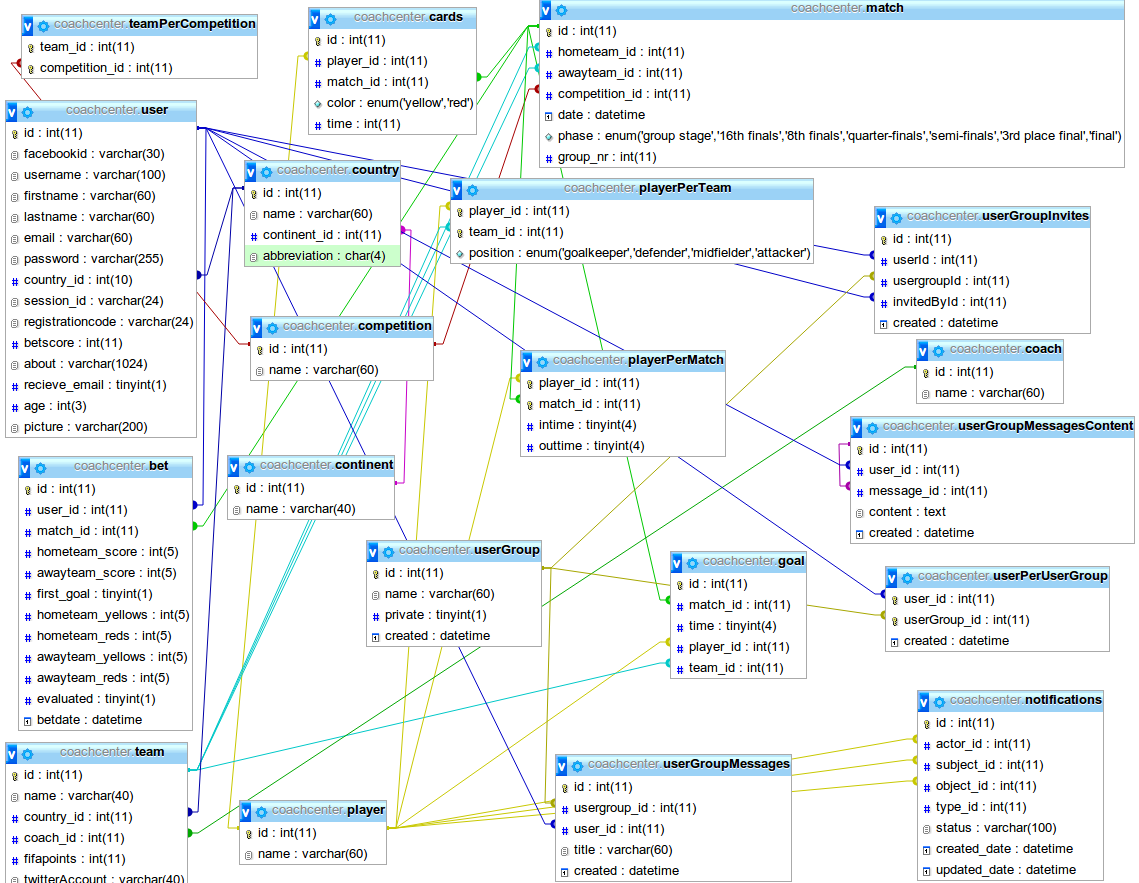
\includegraphics[width=90mm]{ER.png}
%\caption{Onze database in ER-model}
%\label{overflow}
%\end{figure}

\end{document}
